\section{Resultados preliminares}
\label{sec:resultados}

Este capítulo apresenta os resultados obtidos até o momento. O adjetivo
``preliminares'' é literal e tem duas justificativas. A primeira é que o trabalho
reporta, nesta versão, um \emph{único} cenário de estimação: a especificação da
equação~\eqref{eq:principal}, com o corte de período no trimestre do marco e
erros-padrão agrupados por unidade primária de amostragem. Não há aqui bateria
de sensibilidade, estudo de evento nem teste formal de tendências pré-marco, de
modo que os coeficientes devem ser lidos como \textbf{associação condicional}, e
não como estimativas causais do efeito do marco. A segunda é que a agenda de
robustez descrita no Capítulo~\ref{sec:melhorias} (medidas alternativas de
exposição, estimadores alternativos e tratamento do problema de coleta) ainda
não foi executada. O capítulo organiza-se em três blocos: descrição da amostra e
das margens de transição; resultado principal; e síntese.

\subsection{Descrição da amostra e das margens de transição}

A Tabela~\ref{tab:escala} apresenta a escala efetiva de cada domínio de
estimação. O ponto de partida são 3.963.359 pessoas-transições com exposição
atribuída à ocupação de origem, distribuídas por 413 códigos ocupacionais,
31.145 unidades primárias de amostragem e 27 trimestres de origem. Cada desfecho
usa o subconjunto em que está definido, e nenhuma ausência é convertida em zero.

% Gerado por scripts/06_dissertacao.py a partir de output/modelos e output/tabelas.
% Não editar à mão: a próxima execução sobrescreve este arquivo.
\begin{table}[htb]
  \caption{Escala dos domínios de estimação}
  \label{tab:escala}
  \centering
  \espacosimples\idpcorpodez
  \begin{tabular}{@{}lrrrr@{}}
    \toprule
    \textbf{Domínio (desfecho)}                & \textbf{Pessoas-} & \textbf{Células} & \textbf{Ocupa-} & \textbf{UPAs} \\
                                               & \textbf{transições} & \textbf{estimadas} & \textbf{ções} & \\
    \midrule
    Todas as origens (pareamento)              & 3.963.359    & 3.960.584    & 413        & 31.145 \\
    Pares (saída do emprego)                   & 3.178.582    & 3.176.283    & 413        & 31.047 \\
    Destino ocupado (muda de ocupação)         & 2.882.225    & 2.880.049    & 413        & 31.036 \\
    AIOE nos dois lados (margens direcionais)  & 2.879.139    & 2.876.964    & 413        & 31.036 \\
    Origem formal (informalização)             & 1.677.310    & 1.676.862    & 411        & 30.360 \\
    \bottomrule
  \end{tabular}
  \fonte{Elaboração própria a partir da PNADC/IBGE.}
  \nota{Origens de 2019T1 a 2025T3. Pessoas-transições não são pessoas únicas: o
        mesmo indivíduo contribui com até quatro pares. A coluna de células é o
        número de observações efetivamente estimadas em cada modelo.}
\end{table}


A Tabela~\ref{tab:descritivas} traz as médias ponderadas antes e depois do
marco. Três leituras importam. Primeira: as margens direcionais de exposição
sobem quase na mesma proporção (a mobilidade descendente passa de 12,8\% para
17,4\% e a ascendente, de 12,9\% para 17,4\%), o que é compatível com aumento geral das taxas medidas de rotatividade
ocupacional, e não com deslocamento líquido do emprego para ocupações menos
expostas. Segunda: a mudança de ocupação sobe entre sete e oito pontos
percentuais nas duas resoluções, reforçando essa leitura. Terceira: a transição
de formal para informal aumenta cerca de 69\%, de 5,2\% para 8,8\%, movimento
de grande magnitude que exige leitura conjunta
com o ciclo do mercado de trabalho no período. A saída do emprego, em contraste,
praticamente não se move.

% Gerado por scripts/06_dissertacao.py a partir de output/modelos e output/tabelas.
% Não editar à mão: a próxima execução sobrescreve este arquivo.
\begin{table}[htb]
  \caption{Médias ponderadas dos desfechos, antes e depois do marco}
  \label{tab:descritivas}
  \centering
  \espacosimples\idpcorpodez
  \begin{tabular}{@{}lrrr@{}}
    \toprule
    \textbf{Desfecho}                     & \textbf{Pré} & \textbf{Pós} & \textbf{Diferença} \\
    \midrule
    \multicolumn{4}{@{}l}{\textit{Continuidade e vínculo}} \\
    Pareamento entre entrevistas          & 0,783 & 0,812 & $+$0,029 \\
    Saída do emprego                      & 0,079 & 0,081 & $+$0,002 \\
    Transição de formal para informal     & 0,052 & 0,088 & $+$0,036 \\
    \addlinespace
    \multicolumn{4}{@{}l}{\textit{Mobilidade ocupacional}} \\
    Muda de ocupação (2 dígitos)          & 0,209 & 0,280 & $+$0,071 \\
    Muda de ocupação (3 dígitos)          & 0,236 & 0,318 & $+$0,082 \\
    \addlinespace
    \multicolumn{4}{@{}l}{\textit{Gradiente de exposição}} \\
    Transição para menor AIOE             & 0,128 & 0,174 & $+$0,046 \\
    Transição para maior AIOE             & 0,129 & 0,174 & $+$0,046 \\
    \bottomrule
  \end{tabular}
  \fonte{Elaboração própria a partir da PNADC/IBGE.}
  \nota{Pré: origens de 2019T1 a 2022T3. Pós: origens de 2022T4 a 2025T3, pelo
        corte da equação~\eqref{eq:pos}. Médias ponderadas pelo peso amostral da
        entrevista de origem, cada uma no domínio próprio do desfecho.}
\end{table}


A Tabela~\ref{tab:matriz} apresenta a diferença entre as matrizes de mobilidade
pós e pré entre faixas de exposição. O padrão é inequívoco e não é um padrão de
direção: \emph{a permanência na mesma faixa cai em todas as cinco faixas}, entre
3,6 e 8,1 pontos percentuais, com a queda mais forte na quarta faixa. O teste de
Wald da equação~\eqref{eq:wald} rejeita a igualdade das matrizes com estatística
de 3.040,1 e 20 graus de liberdade. A Figura~\ref{fig:matriz} apresenta a mesma
informação em forma gráfica.

% Gerado por scripts/06_dissertacao.py a partir de output/modelos e output/tabelas.
% Não editar à mão: a próxima execução sobrescreve este arquivo.
\begin{table}[htb]
  \caption{Diferença entre as matrizes de mobilidade pós e pré, por faixa de exposição}
  \label{tab:matriz}
  \centering
  \espacosimples\idpcorpodez
  \begin{tabular}{@{}lrrrrr@{}}
    \toprule
    \textbf{Faixa de origem} & \multicolumn{5}{c}{\textbf{Faixa de destino (p.p.)}} \\
    \cmidrule(l){2-6}
     & \textbf{Q1} & \textbf{Q2} & \textbf{Q3} & \textbf{Q4} & \textbf{Q5} \\
    \midrule
    Q1 (menor exposição) & $-$3,60  & $+$2,03  & $+$1,04  & $+$0,34  & $+$0,19 \\
    Q2                   & $+$2,05  & $-$4,97  & $+$1,60  & $+$0,75  & $+$0,57 \\
    Q3                   & $+$1,17  & $+$1,83  & $-$6,42  & $+$1,55  & $+$1,87 \\
    Q4                   & $+$0,69  & $+$1,22  & $+$2,46  & $-$8,06  & $+$3,69 \\
    Q5 (maior exposição) & $+$0,26  & $+$0,82  & $+$1,92  & $+$2,78  & $-$5,79 \\
    \bottomrule
  \end{tabular}
  \fonte{Elaboração própria a partir da PNADC/IBGE.}
  \nota{Faixas fixas entre códigos ocupacionais. Erros-padrão por reamostragem
        de UPA (199 réplicas) variam entre 0,04 e 0,28 p.p.; todas as células
        têm intervalo de 95\% que exclui zero. Teste de Wald de igualdade das
        matrizes: $\chi^2 = 3.040{,}1$, 20 graus de liberdade.}
\end{table}


\begin{figure}[htb]
  \caption{Diferença entre as matrizes de mobilidade pós e pré}
  \label{fig:matriz}
  \centering
  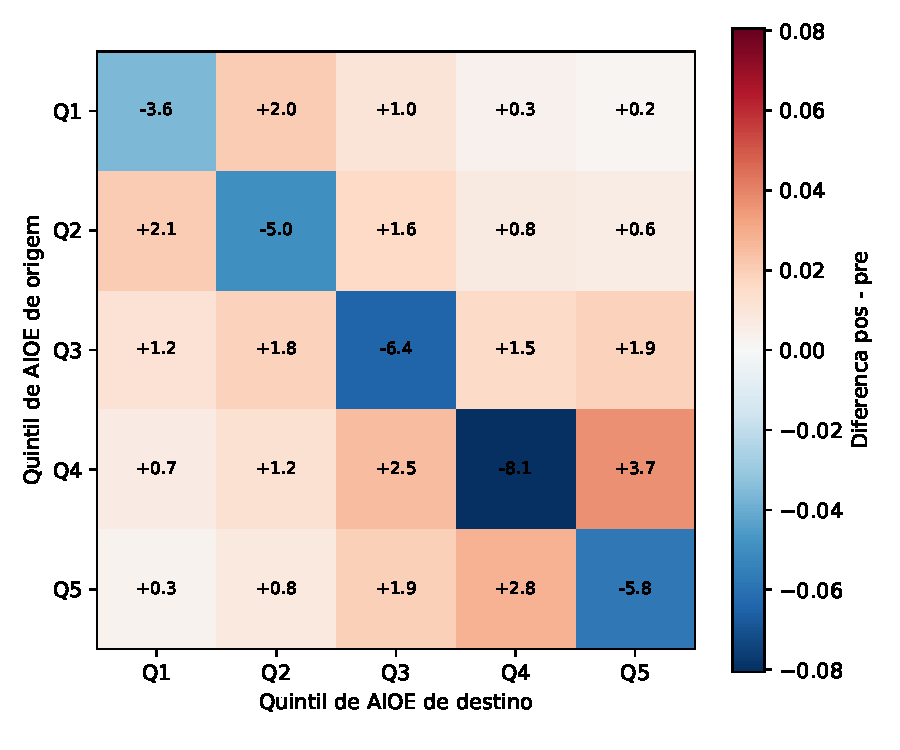
\includegraphics[width=0.85\textwidth]{figuras/fig_matriz_diferencas.pdf}
  \fonte{Elaboração própria a partir da PNADC/IBGE.}
\end{figure}

Um achado descritivo adicional merece registro porque condiciona toda a leitura
temporal. A taxa ponderada de mudança de código ocupacional em três dígitos
entre entrevistas consecutivas cai abruptamente de 30,0\% nas origens de 2019T4
para 15,3\% nas de 2020T1, permanece entre 13\% e 15\% durante todo o período de
coleta telefônica e retorna a 34,3\% nas origens de 2021T4. Essa
descontinuidade coincide com as mudanças no modo de coleta da pesquisa
\parencite{ibge2022tratamento}, o que torna plausível um problema de medida. Os
dados aqui apresentados, porém, não separam o efeito da coleta de mudanças reais
do mercado de trabalho na pandemia, de alterações de composição amostral, do
atrito e da codificação ocupacional. Tampouco a comparação entre a magnitude
dessa quebra agregada e a dos coeficientes demonstra, por si, viés no gradiente:
para isso seria preciso verificar se a quebra varia com a exposição. Como o
desenho desta versão usa a série inteira, parte do contraste entre pré e pós
atravessa essa descontinuidade, razão pela qual seu tratamento encabeça a agenda
do Capítulo~\ref{sec:melhorias}.

\subsection{Resultado principal}

A Tabela~\ref{tab:principal} apresenta os coeficientes da
equação~\eqref{eq:principal} para os sete desfechos, em pontos percentuais por unidade de AIOE da ocupação de origem (cerca de um
desvio-padrão entre ocupações; Seção~\ref{sec:exposicao}). O painel A traz o coeficiente
de interesse $\beta$, sobre a interação entre exposição e período; o painel B
traz o coeficiente $\gamma$ da teletrabalhabilidade interagida com o período,
estimado simultaneamente na mesma equação. A Figura~\ref{fig:coeficientes}
apresenta o painel A em forma gráfica.

% Gerado por scripts/06_dissertacao.py a partir de output/modelos e output/tabelas.
% Não editar à mão: a próxima execução sobrescreve este arquivo.
\begin{table}[htb]
  \caption{Gradiente de exposição e de teletrabalhabilidade, cenário único}
  \label{tab:principal}
  \centering
  \espacosimples\idpcorpodez
  \begin{tabular}{@{}lrrlr@{}}
    \toprule
    \textbf{Desfecho}                  & \textbf{Efeito (p.p.)} & \textbf{E.P.} & \textbf{IC 95\%}       & \textbf{$p$} \\
    \midrule
    \multicolumn{5}{@{}l}{\textit{Painel A --- Exposição $\times$ pós}} \\
    \addlinespace[2pt]
    Transição para menor AIOE          & $+$2,187  & 0,105 & [$+$1,982; $+$2,393]   & $<$0,001 \\
    Muda de ocupação (3 dígitos)       & $+$0,861  & 0,136 & [$+$0,594; $+$1,128]   & $<$0,001 \\
    Muda de ocupação (2 dígitos)       & $+$0,278  & 0,128 & [$+$0,027; $+$0,529]   & 0,030 \\
    Saída do emprego                   & $-$0,250  & 0,075 & [$-$0,398; $-$0,103]   & $<$0,001 \\
    Pareamento (teste de atrito)       & $-$0,261  & 0,141 & [$-$0,536; $+$0,015]   & 0,064 \\
    Transição de formal para informal  & $-$0,673  & 0,094 & [$-$0,858; $-$0,488]   & $<$0,001 \\
    Transição para maior AIOE          & $-$1,364  & 0,103 & [$-$1,566; $-$1,161]   & $<$0,001 \\
    \addlinespace
    \multicolumn{5}{@{}l}{\textit{Painel B --- Teletrabalhabilidade $\times$ pós}} \\
    \addlinespace[2pt]
    Transição para menor AIOE          & $-$0,239  & 0,255 & [$-$0,739; $+$0,262]   & 0,350 \\
    Muda de ocupação (3 dígitos)       & $+$0,093  & 0,309 & [$-$0,512; $+$0,698]   & 0,763 \\
    Muda de ocupação (2 dígitos)       & $+$0,391  & 0,290 & [$-$0,178; $+$0,960]   & 0,178 \\
    Saída do emprego                   & $+$0,215  & 0,153 & [$-$0,086; $+$0,515]   & 0,161 \\
    Pareamento (teste de atrito)       & $-$0,362  & 0,291 & [$-$0,932; $+$0,208]   & 0,213 \\
    Transição de formal para informal  & $+$1,734  & 0,199 & [$+$1,345; $+$2,124]   & $<$0,001 \\
    Transição para maior AIOE          & $+$0,762  & 0,221 & [$+$0,330; $+$1,195]   & $<$0,001 \\
    \bottomrule
  \end{tabular}
  \fonte{Elaboração própria a partir da PNADC/IBGE.}
  \nota{Efeito em pontos percentuais por desvio-padrão de exposição da ocupação
        de origem, no painel A, e por unidade do índice de teletrabalhabilidade,
        no painel B. Os dois painéis vêm da mesma estimação. Erros-padrão
        agrupados por UPA, entre 30.360 e 31.145 grupos conforme o domínio. O
        desfecho de pareamento é um teste de atrito: não rejeitar é o resultado
        desejável.}
\end{table}


\begin{figure}[htb]
  \caption{Gradiente de exposição por desfecho, com intervalos de 95\%}
  \label{fig:coeficientes}
  \centering
  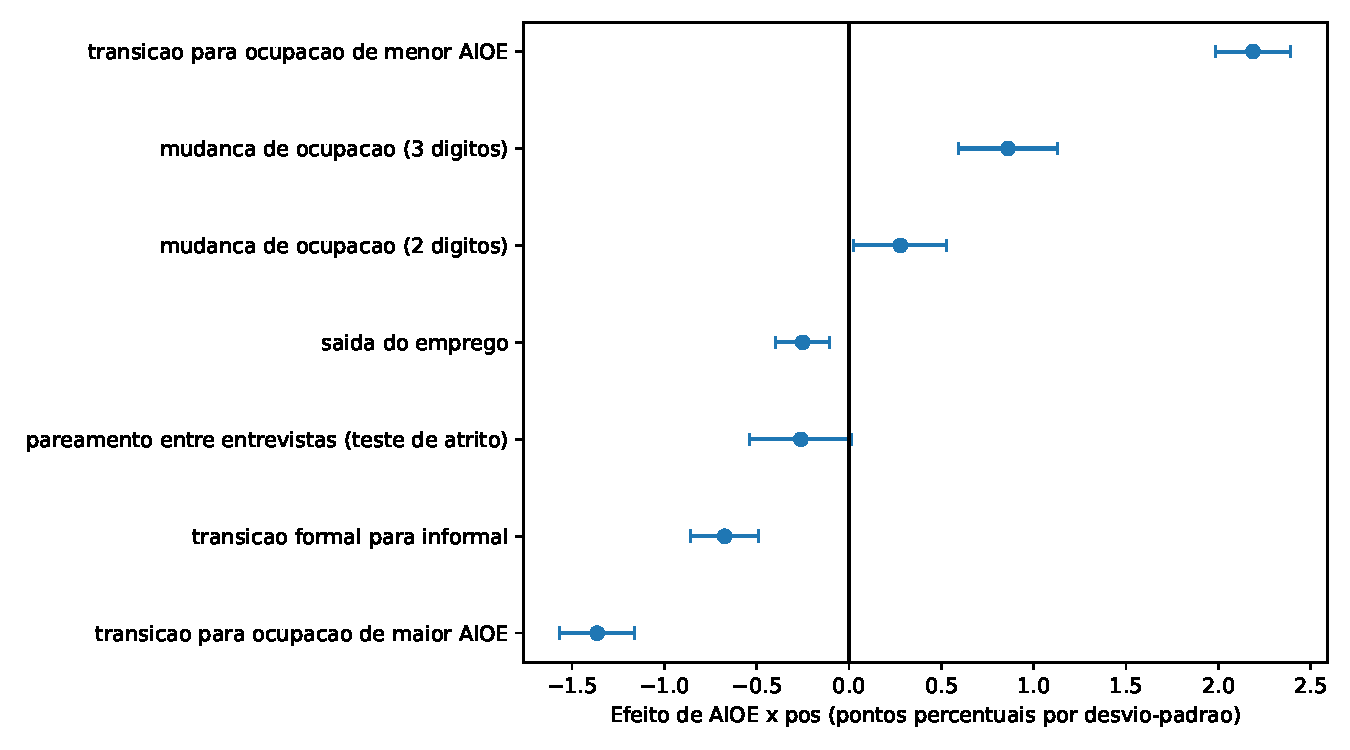
\includegraphics[width=0.92\textwidth]{figuras/fig_coeficientes_aioe.pdf}
  \fonte{Elaboração própria a partir da PNADC/IBGE.}
  \nota{Efeito da interação entre exposição e período, em pontos percentuais por
        unidade de AIOE da ocupação de origem.}
\end{figure}

A leitura literal é a seguinte. Condicionalmente aos efeitos fixos de ocupação
de origem e de UF-trimestre, à teletrabalhabilidade interagida com o período e
ao conjunto de covariáveis demográficas e contratuais, a mudança entre o período
pré e o pós na probabilidade de transitar para ocupação menos exposta é 2,19
pontos percentuais maior para ocupações de origem com uma unidade a mais de
AIOE; na probabilidade de transitar para ocupação mais exposta, a mudança é 1,36
ponto percentual menor. O coeficiente compara, portanto, as mudanças entre pré e
pós de ocupações com exposições diferentes, e não acompanha uma mesma ocupação
cuja exposição aumente, já que o AIOE é constante dentro de cada ocupação.

Esses dois números precisam ser lidos em conjunto e contra o pano de fundo
descritivo. As duas margens direcionais subiram \emph{ambas} cerca de 4,6 pontos
percentuais entre os períodos, conforme a Tabela~\ref{tab:descritivas}. O que os
coeficientes acrescentam é que essa subida geral não foi simétrica ao longo do
gradiente: entre ocupações de origem, quanto maior a exposição, mais a
composição do movimento pendeu para o lado descendente. Essa assimetria, porém,
não é necessariamente específica à exposição: como discutido na
Seção~\ref{sec:desfechos}, origens mais expostas têm mais destinos possíveis
abaixo delas, e um aumento geral de mobilidade tende, por si só, a elevar mais
sua mobilidade descendente, canal que o desenho atual não separa do gradiente.
Em magnitude, o coeficiente corresponde a cerca de 12,6\% da taxa pós de
transição para ocupação menos exposta (2,19 pontos percentuais sobre 17,4\%).

O terceiro grupo de resultados é o de frequência de mudança. Maior exposição
associa-se a mais mudança de ocupação, com $+0{,}86$ ponto percentual na
resolução de três dígitos e $+0{,}28$ na de dois dígitos. A diferença entre as duas resoluções sugere que parte do movimento adicional
associado à exposição ocorre \emph{dentro} das categorias de dois dígitos da
COD, e não entre elas; uma inferência formal sobre essa diferença exigiria
considerar a covariância entre as duas estimativas.

O quarto grupo é o das margens de vínculo, e o sinal é contraintuitivo. Maior
exposição associa-se a \emph{menos} saída do emprego ($-0{,}25$ ponto
percentual) e a \emph{menos} transição de formal para informal ($-0{,}67$ ponto
percentual). Isto é, no período analisado, trabalhadores em ocupações mais
expostas não apresentaram deterioração relativa de vínculo; se algo, o contrário.
Nesse desfecho, o coeficiente da teletrabalhabilidade é positivo e expressivo
($+1{,}73$ ponto percentual por unidade do índice, painel B), enquanto o da
exposição é negativo. Como os dois índices têm escalas distintas, os
coeficientes não são diretamente comparáveis em magnitude: o desenho permite
relatar os dois gradientes condicionais, mas não identificar qual força explica
o aumento agregado da informalização.

O teste de atrito merece nota específica. O coeficiente sobre a probabilidade de
pareamento é $-0{,}261$ ponto percentual, com $p = 0{,}064$: não se rejeita a hipótese de que o gradiente de pareamento em relação à
exposição tenha permanecido estável entre os períodos, mas o resultado está
próximo do limiar convencional e o sinal é negativo. Como diferenças
permanentes de retenção entre ocupações são absorvidas pelo efeito fixo, o teste
também não as avalia. Isso não invalida os demais desfechos, mas impede afirmar
que a seleção longitudinal esteja descartada.

Uma ressalva de leitura fecha a seção. São sete desfechos fortemente
correlacionados, estimados sobre a mesma base e com a mesma especificação, sem
correção para multiplicidade. O coeficiente de mudança de ocupação em dois
dígitos, com $p = 0{,}030$, é o que menos resiste a essa ressalva e não deve ser
citado isoladamente.

\subsection{Síntese dos resultados preliminares}

Os resultados preliminares sustentam quatro afirmações, e apenas quatro.

\textbf{Primeira.} Houve aumento generalizado das taxas medidas de rotatividade
ocupacional na amostra entre o período pré e o pós, visível na queda de
permanência em \emph{todas} as faixas de exposição e na subida simultânea das
duas margens direcionais. Parte relevante desse movimento é comum às ocupações,
o que não exclui a participação de mecanismos associados à exposição.

\textbf{Segunda.} Condicionalmente à ocupação de origem, ao par UF-trimestre, à
teletrabalhabilidade interagida com o período e ao conjunto de controles, há
gradiente estatisticamente detectável associado à exposição: maior exposição
associa-se a mais transições para ocupações menos expostas, menos transições
para ocupações mais expostas e mais mudança de ocupação, sobretudo de resolução
fina. A magnitude é da ordem de dois pontos percentuais por unidade de AIOE, cerca
de um oitavo da taxa pós de transição para ocupação menos exposta. Nas margens
direcionais, esse gradiente não está separado do canal mecânico descrito na
Seção~\ref{sec:desfechos}.

\textbf{Terceira.} Nas margens de vínculo o sinal é o oposto do que a leitura
alarmista sobre inteligência artificial anteciparia: maior exposição associa-se a
menos saída do emprego e a menos informalização. Na informalização, o gradiente é negativo em relação à exposição e positivo em
relação à teletrabalhabilidade, sem que o desenho identifique qual força explica
o aumento agregado.

\textbf{Quarta, e limitante.} Nada disso é evidência causal. O desenho reporta um
único cenário, sem estudo de evento, sem teste de tendências pré-marco e sem
bateria de sensibilidade; a série usada atravessa uma descontinuidade na taxa medida de mudança de
ocupação em 2020 e 2021, coincidente com a mudança no modo de coleta e de causa
ainda não demonstrada. Os coeficientes da Tabela~\ref{tab:principal}
devem ser lidos como descrição condicional de um período que contém essa
descontinuidade. O Capítulo~\ref{sec:melhorias} organiza o que precisa ser feito
para mudar esse diagnóstico, e coloca o tratamento do problema de coleta como
prioridade.
